\subsection{Autonomy and Software}
\label{sec:autonomy-and-software}

Project: Icarus incorporates a large amount of software for command and control, flight
compute subsystems and attitude, in-flight path and system management. These elements
run on a Linux-based ground station, an onboard NVIDIA Jetson TX2i, and ZeroPilot 3.0, a
custom flight computer.

\begin{figure}[H]
        \centering
        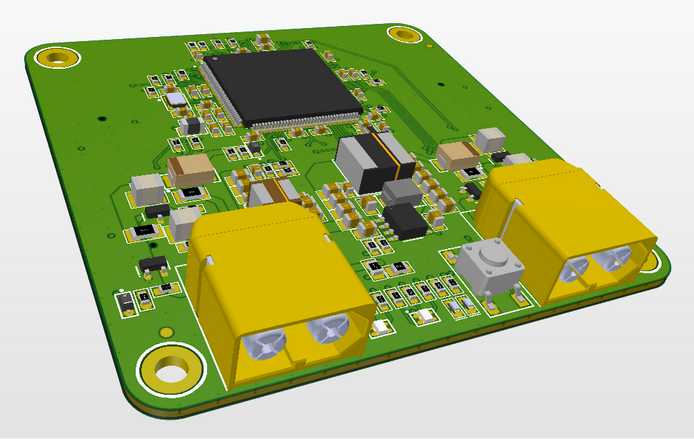
\includegraphics[scale=0.4]{pcb}
        \caption{ZeroPilot 3.0 flight controller PCB design}
\end{figure}

\subsubsection{Command and Control}
\label{sec:command-and-control}

Command and Control is handled by a software system called IMACS (Integrated Monitoring
And Control System). It supports three direct wireless RF links between the operational
team and the aircraft:
\begin{itemize}
    \item 900 MHz Command and Control Link
    \item 1.2 GHz Video Receiver
    \item LTE Backup Control and Monitoring Link
\end{itemize}

\begin{figure}[h]
        \centering
        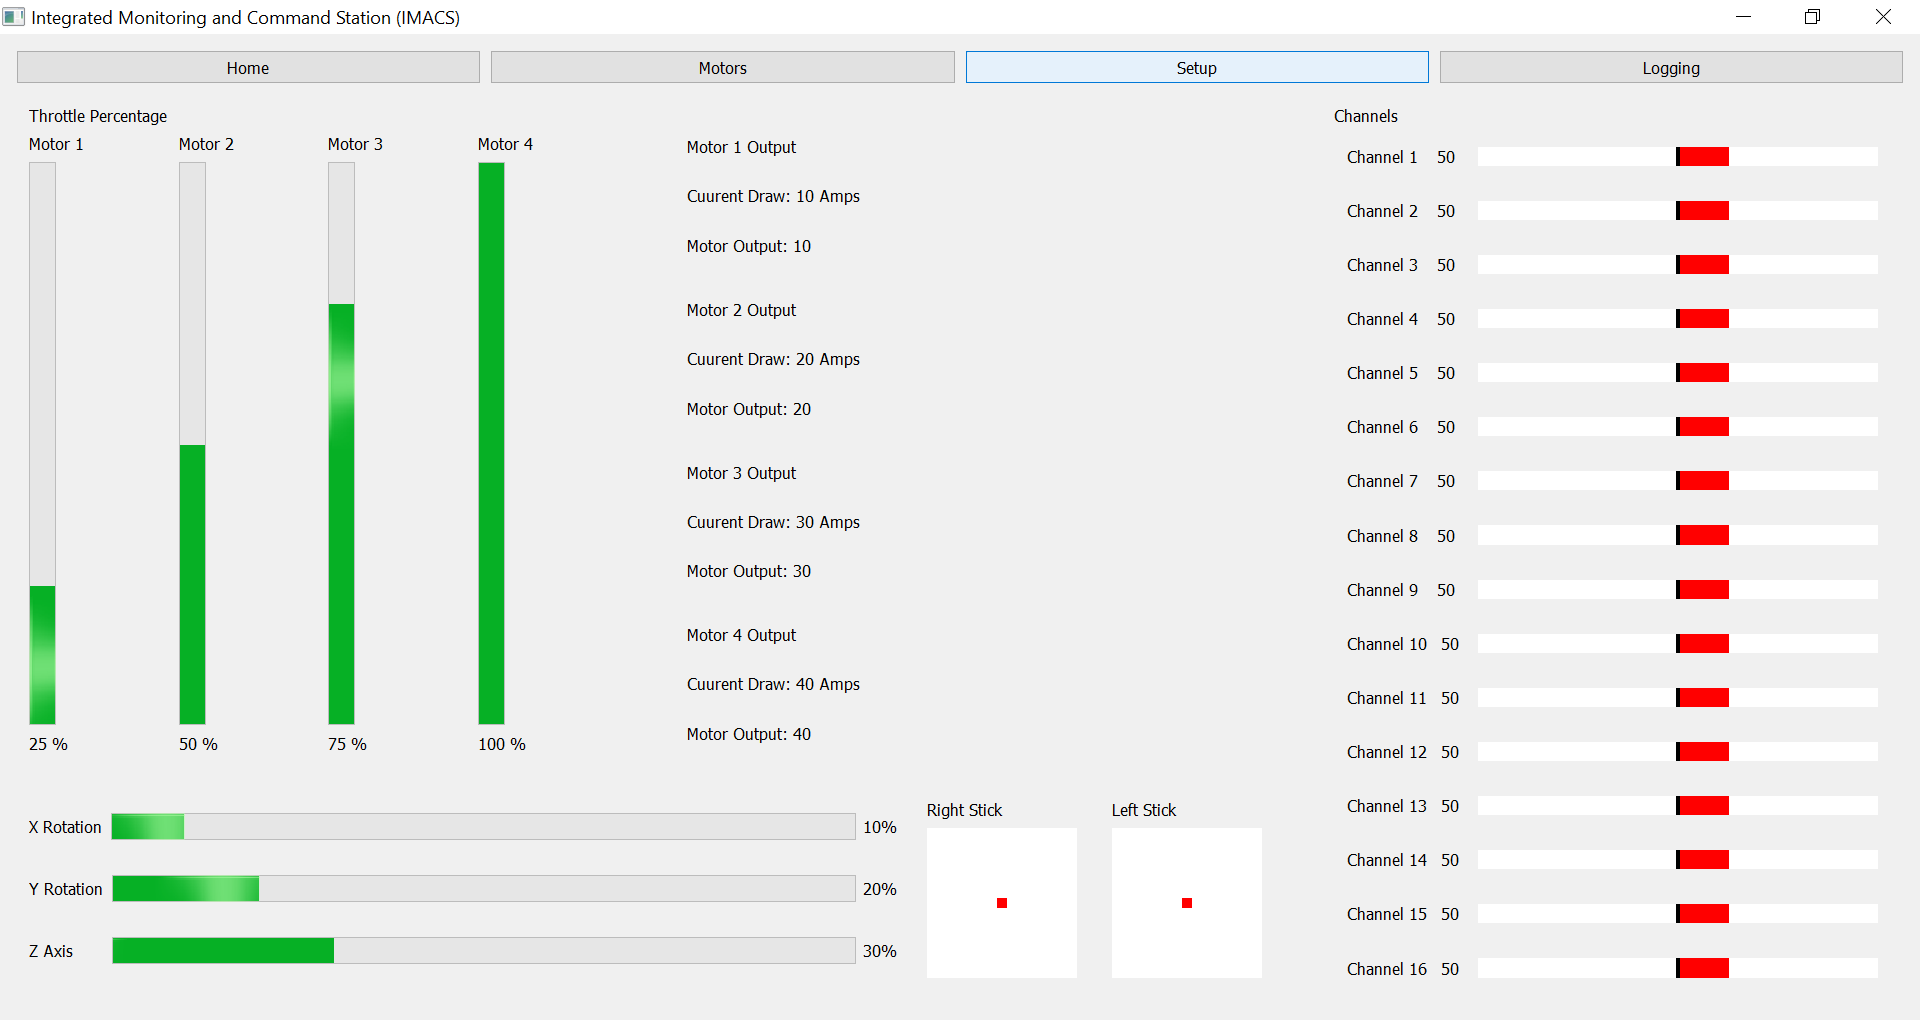
\includegraphics[scale=0.40]{imacs-outputs}
        \caption{IMACS Setup page for monitoring aircraft attitude and power usage.}
\end{figure}

Using a desktop interface written in Python with QT, IMACS is able to display the
state of the aircraft, including the GPS position, airspeed, monitor battery levels, 
power draw, attitude, motor outputs, jitter and a low-latency analog video feed. IMACS
also offers the ability for a pilot to remotely plan and sequence waypoints with
automatic return-to-home and seamless tele-operated handover.

\begin{figure}[H]
        \centering
        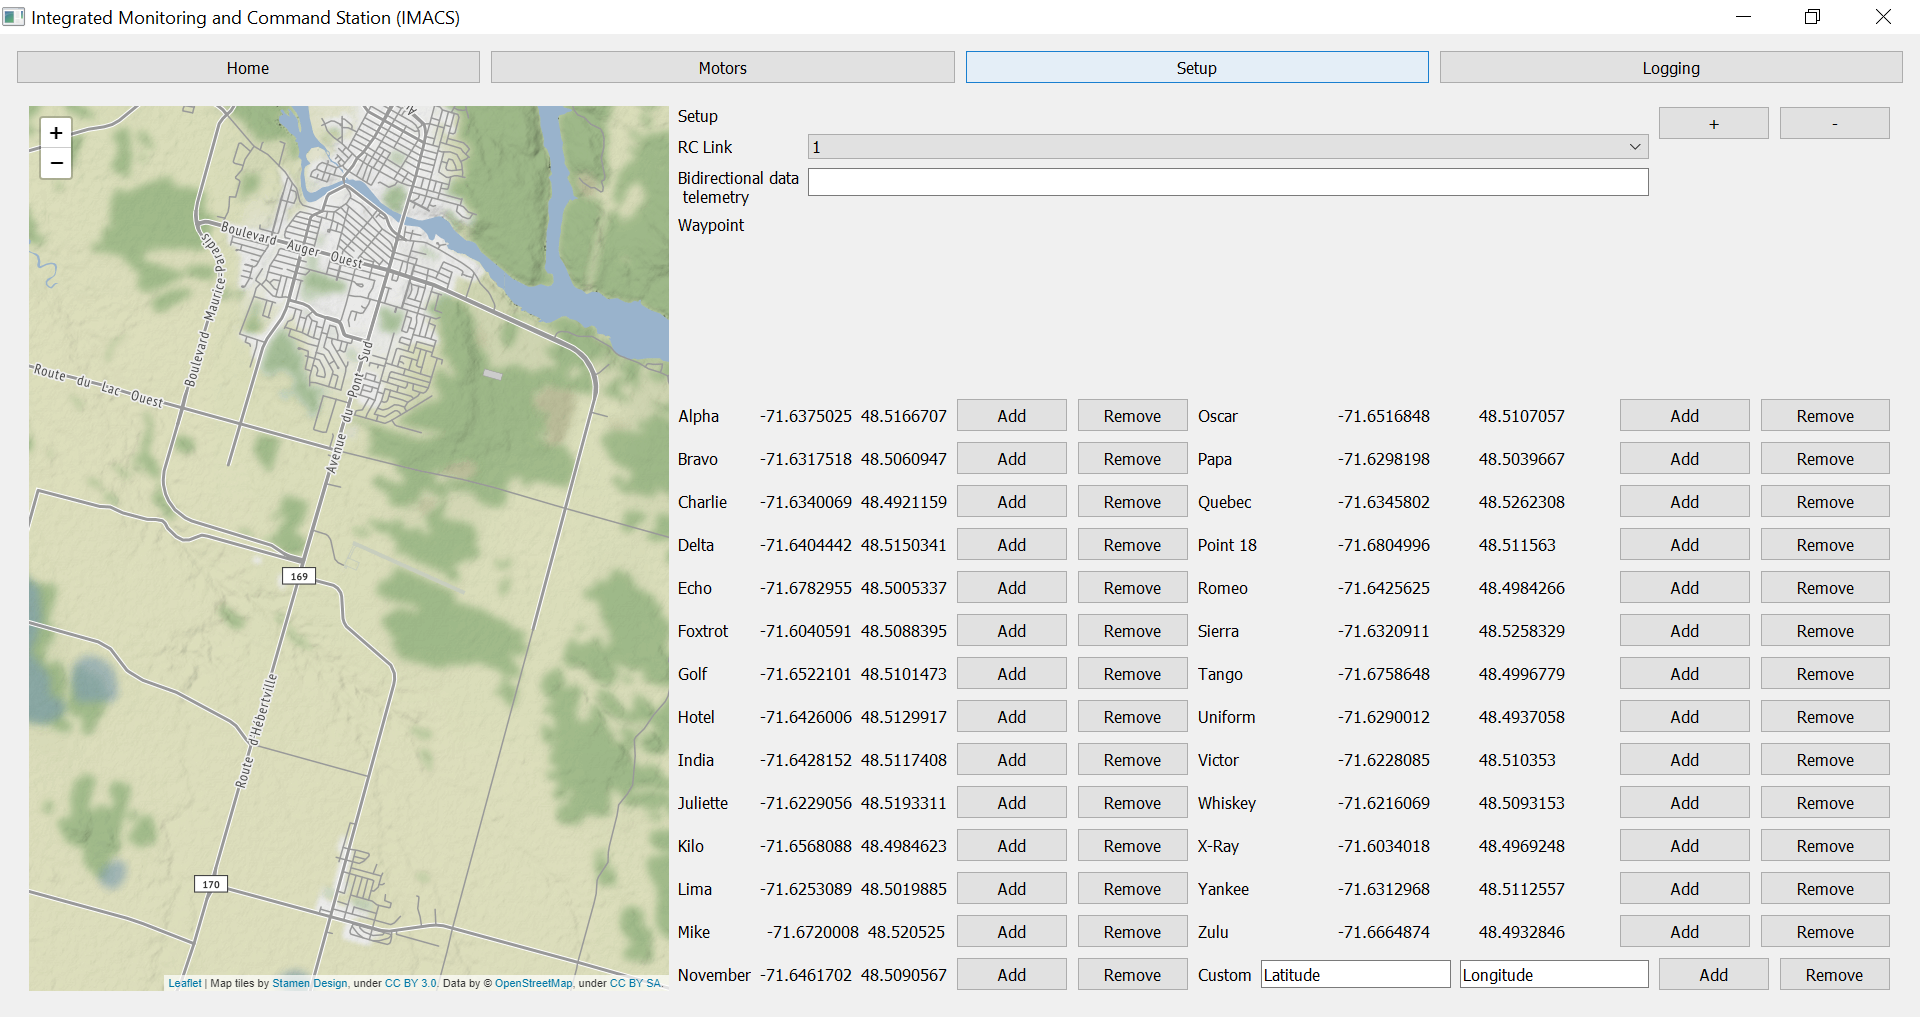
\includegraphics[scale=0.40]{imacs-waypoints}
        \caption{IMACS waypoint management and selection interface.}
\end{figure}

IMACS provides numerous distinct advantages over traditional Ground Control Software
such as Mission Planner or QGround Control. One key feature is the ability to define
a custom message protocol, which allows for greater flexibility and control over the
aircraft's communication and navigation. Additionally, IMACS offers a more customizable
approach to defining competition-specific aspects such as waypoints and overall path.
This gives the pilot significantly more control over the precise flight, which helps
improve efficiency during flight as well as the ability to divert in the case of
an emergency. The user interface of IMACS is designed with Project: Icarus in mind,
providing a simplified and user-friendly interface.

\subsubsection{Flight Compute}
\label{sec:flight-compute}

Flight computer and avionics is all handled on-board the STM32L5 based ZeroPilot 3.0
PCB. WARG has decided to pair the "LaminarOS" operation system with the 3rd major
revision of ZeroPilot software. The custom software and firmware stack allows
the use of a significantly lower power flight stack on an L5 chip (compared to traditional
F4, F7 or H7 chips in commercially available boards), as well as allowing for more 
flexibility in future revisions and updates of ZeroPilot.

\paragraph{LaminarOS}

LaminarOS (LOS) is WARG's custom middleware software that consists of 3 major parts,
LOS Interface, LOS Drivers and LOS Core, allowing for useful abstraction and
portability across multiple platforms and projects. LOS Interface provides software
interface for any application/control to drivers, hiding unnecessary implementation
details. This abstraction allows for both the application software and drivers to be
portable across any project. LOS Drivers provide drivers for all sensors and 
peripherals, exposing simple interfaces of any application using it. Finally, LOS Core
provides wrapper functions for any board support packages made available from chip
manufacturers, in this case, STM32's HAL.

\begin{figure}[H]
        \centering
        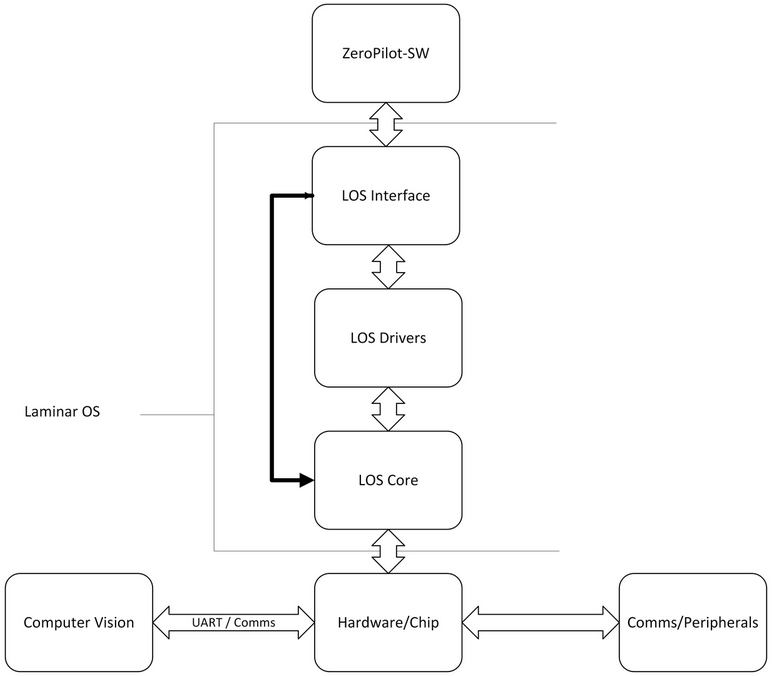
\includegraphics[scale=0.5]{los}
        \caption{LaminarOS architecture diagram}
\end{figure}

\paragraph{ZeroPilot Software 3.0}

ZeroPilot runs on top of LaminarOS, and starts on book with the \textit{System 
Manager} state machine, which handles the drone operating state. This includes:
\begin{itemize}
    \item \textbf{Boot}: runtime configuration, initialization, GPS lock, sensor 
    calibrations
    \item \textbf{Disarm}: UAS is disarmed and in low power mode. Flight plans can be
    sequenced.
    \item \textbf{Ground Operations}: UAS is operating and moving, but no the ground
    \item \textbf{Flight}: Aircraft is fully armed and capable of pursuing any action
    in the decision tree
    \item \textbf{Failure}: Failsafe mode for safety. The aircraft will not exit from
    this without restarting.
\end{itemize}


\begin{figure}[H]
        \centering
        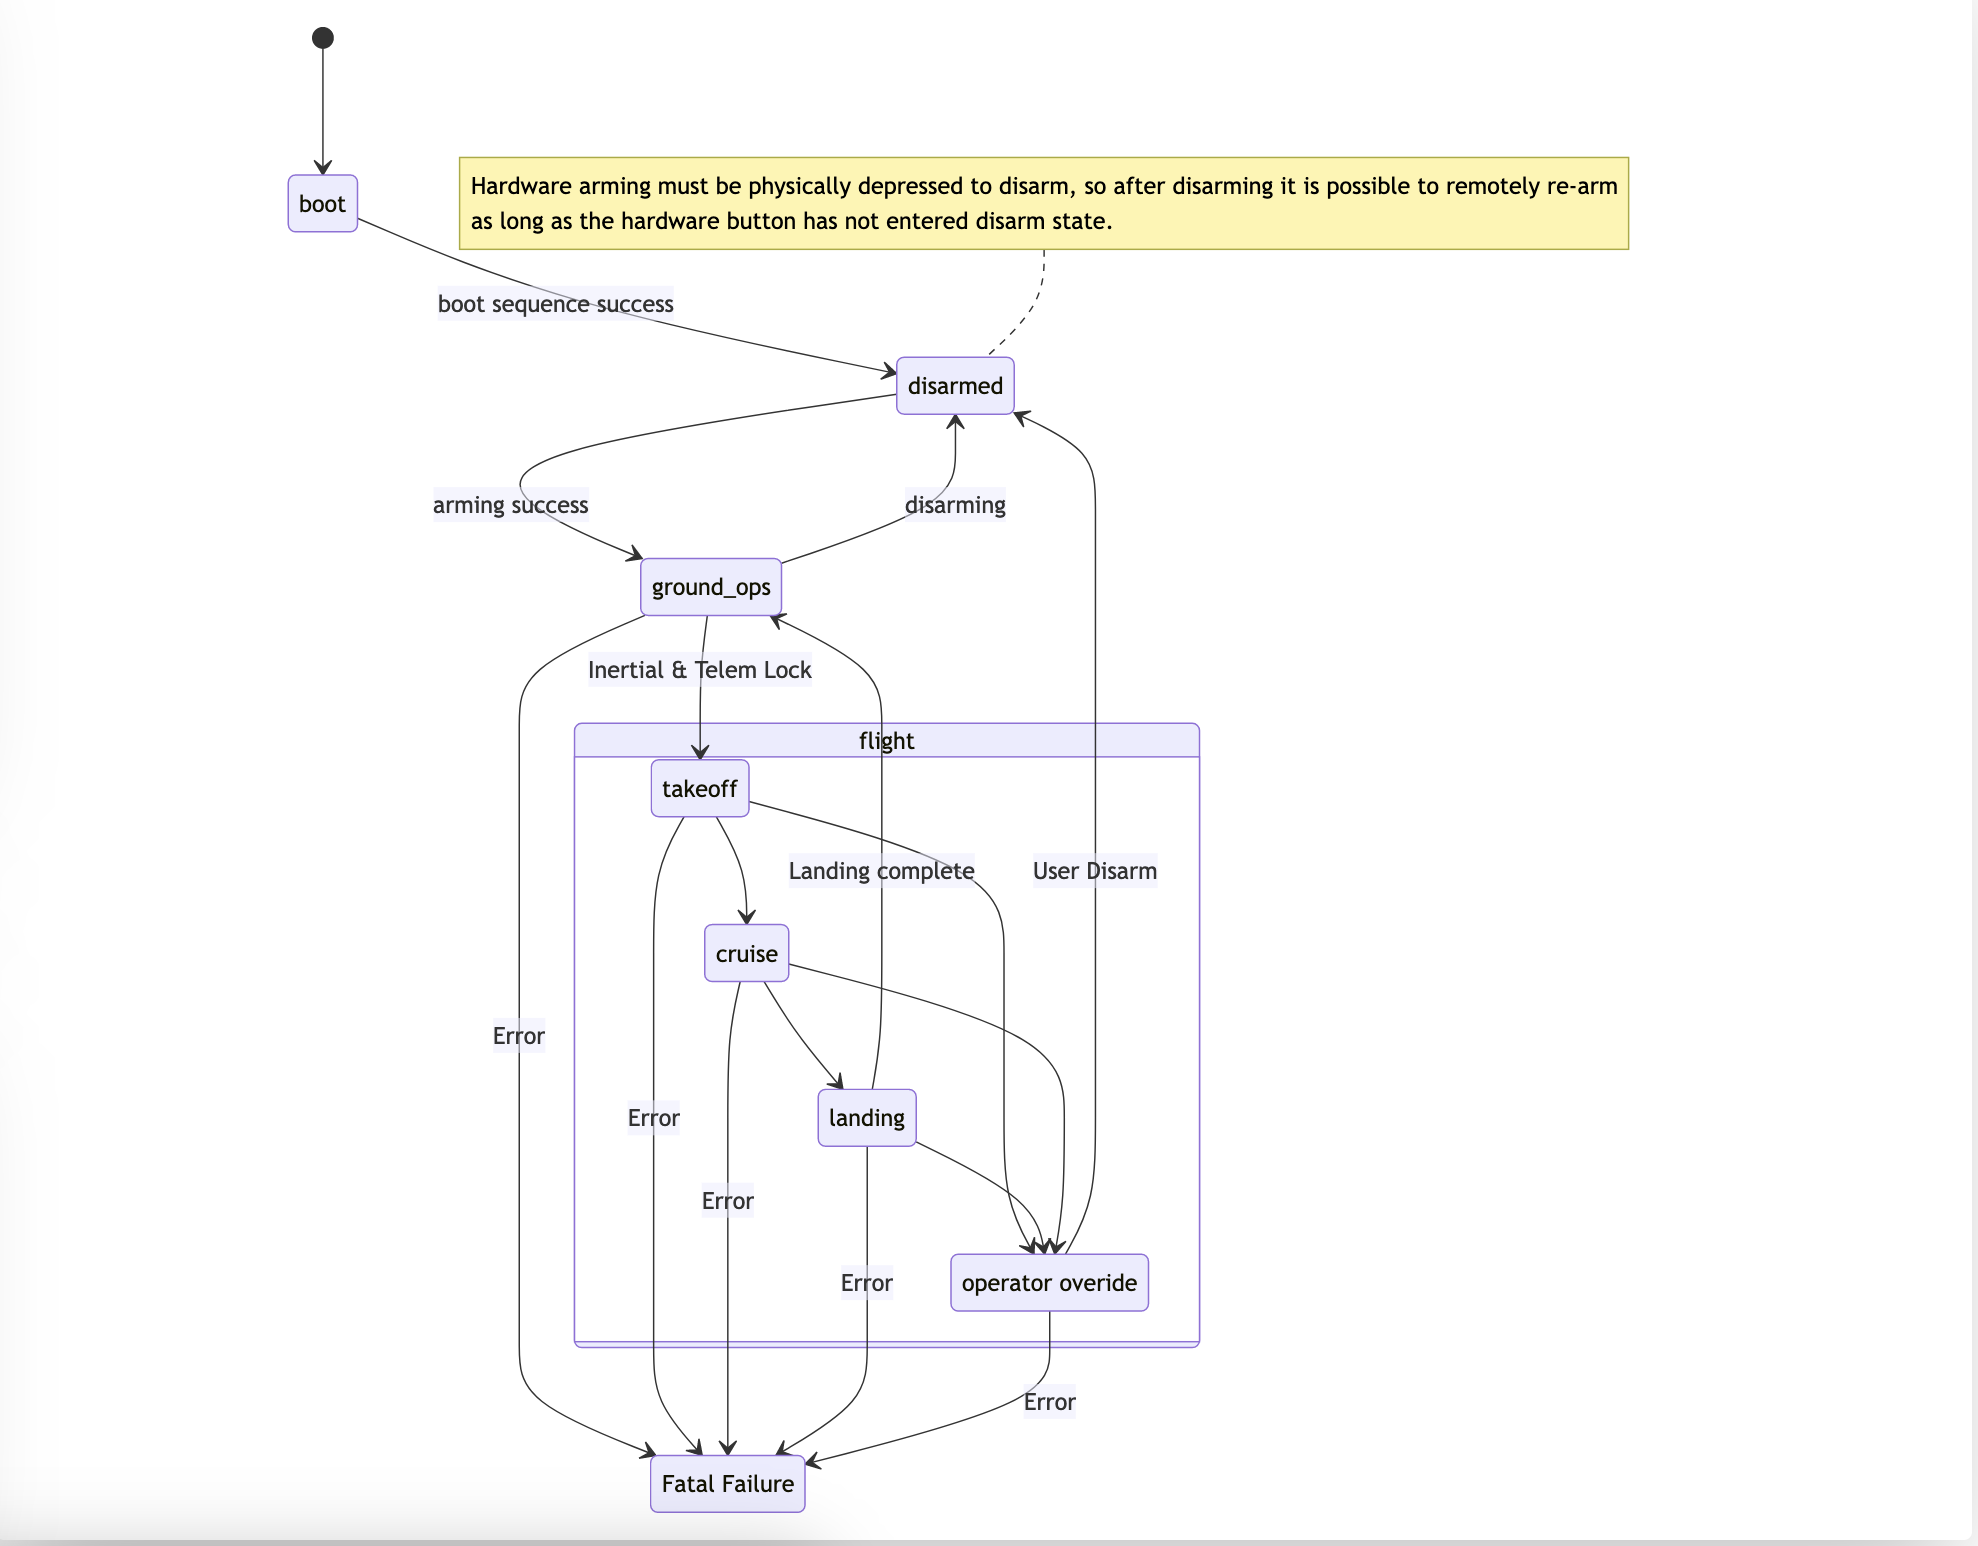
\includegraphics[scale=0.15]{sm-arch}
        \caption{\textit{System Manager}'s state machine decision tree}
\end{figure}

In each of these states, \textit{System Manager} (SM) will leverage the functionality 
of the sub-module managers: \textit{Attitude Manager, Path Manager and Telemetry 
Manager} to either follow commands from the ground station, or the pilot. In all 
cases, SM consolidates incoming data from \textit{Telemetry Manager} to consistent 
data formats for \textit{Path Manager} and \textit{Attitude Manager}. This means that 
all software modules are incredibly portable since they have a common interface to SM.

\textit{Attitude Manager} (AM) is an event loop which handles the attitude control of
the aircraft by running a series of finely-tuned closed-loop control algorithms on a
simplified state-space model. This allows AM to handle real-time changes in the
aircraft's control surfaces, or changes to the balance of the aircraft. The use of
a proprietary state-space model also means that any aircraft can be modelled in a
linear relation to each actuator, allowing for great adaptability between different
airframes or airframe configurations. The closed-loop controls algorithms run at a
fixed 100 Hz, based on a movement vector received from either the pilot or
\textit{Path Manager}.

\textit{Path Manager} (PM) is a state machine that sequences commands on the fly to
waypoints, takeoff, or land autonomously. PM will retrieve instructions and the
aircraft's current position data from SM. PM will then pass ascent and descent
velocity targets along to AM to use accordingly. PM uses a list of waypoints, given
by SM, as well as the aircraft's current position, to calculate the required movement
vector and heading that will allow the UAS to fly to the next waypoint. It performs
these calculations and sends the resulting data to AM for each waypoint within the
list. If there is a need to reroute, this list will be updated and sent to PM for
it to update its calculations.

\textit{Telemetry Manager} (TM) is an event loop that handles all software I/O on the
aircraft. TM is responsible for communication with the Jetson as well as the ground
station. TM interfaces with LOS' UART driver for communication with the Jetson and
LOS' RFD900x driver for sending messages to and from the ground. The Lightweight
Communications and Marshalling (LCM) code generator is used to generate C++ code
for each type of message payload as well as helper functions for message
serialization. On each loop, TM will read incoming data from SM and assemble message
structs to send to the appropriate device. It then marshals the structs to bytes and 
uses LOS to interface with the corresponding device.